\documentclass[border=0mm]{standalone}
\usepackage{pgfplots}
\usepgfplotslibrary{groupplots}
\pgfplotsset{compat=1.17}
\usepackage{xcolor}
\usepackage{xstring}
\usepackage{tikz}
\usepackage{eqparbox}


\definecolor{color1}{rgb}{0,0.4470,0.7410}
\definecolor{color2}{rgb}{0.8500,0.3250,0.0980}
\definecolor{color3}{rgb}{0.9290,0.6940,0.1250}
\definecolor{color4}{rgb}{0.4940,0.1840,0.5560}
\definecolor{color5}{rgb}{0.4660,0.6740,0.1880}
\definecolor{color6}{rgb}{0.3010,0.7450,0.9330}


\begin{document}

\pgfplotsset{
compat=1.11,
legend image code/.code={
\draw[mark repeat=2,mark phase=2]
plot coordinates {
(0cm,0cm)
(0.3cm,0cm)        %% default is (0.3cm,0cm)
(0.6cm,0cm)         %% default is (0.6cm,0cm)
};%
}
}%

\pgfdeclarelayer{background layer}%
\pgfdeclarelayer{foreground layer}%
\pgfsetlayers{background layer,main,foreground layer}%

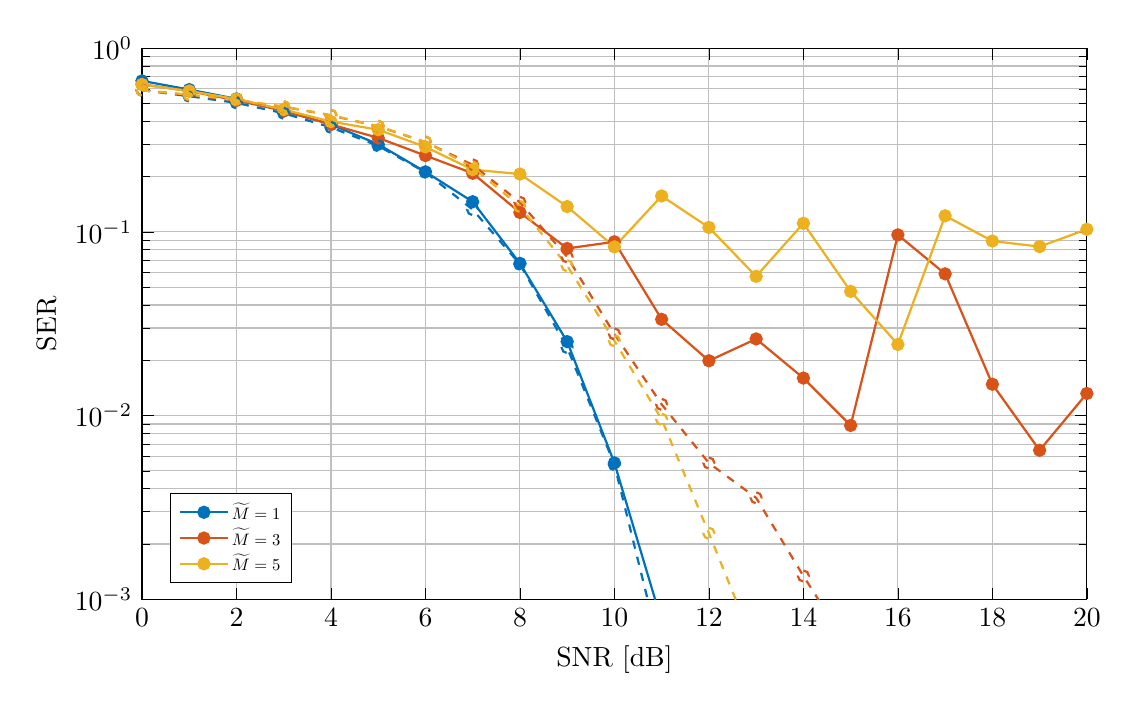
\begin{tikzpicture}[
]
\begin{semilogyaxis}[%
width=12cm,
height=7cm,
scale only axis,
every outer x axis line/.append style={black},
every x tick label/.append style={font=\color{black}},
every x tick/.append style={black},
xmin=0,
xmax=20,
xlabel={SNR [dB]},
every outer y axis line/.append style={black},
every y tick label/.append style={font=\color{black}},
every y tick/.append style={black},
ymin=0.001,
ymax=1,
ylabel={SER},
axis background/.style={fill=white},
xmajorgrids,
ymajorgrids,
yminorgrids,
xtick={0,2,...,20},
legend pos=south west,
legend style={nodes={scale=0.6, transform shape}},
legend cell align={left},
]

\addplot [thick,color1, mark=*] coordinates {(0,0.6637700796127319)(1,0.5950496792793274)(2,0.5299700498580933)(3,0.45496025681495667)(4,0.38466987013816833)(5,0.29976990818977356)(6,0.212289959192276)(7,0.1459599733352661)(8,0.06741001456975937)(9,0.02528000995516777)(10,0.005530005786567926)(11,0.0007600002572871745)(12,7.000000186963007e-05)(13,2.0000001313746907e-05)(14,3.0000002880115062e-05)(15,0.0001800000318326056)(16,0.0)(17,0.0)(18,0.0)(19,0.0)(20,0.0)};
\addlegendentry{$\widetilde{M}=1$}

\addplot [thick,color2, mark=*] coordinates {(0,0.6353999972343445)(1,0.5840299129486084)(2,0.5194100737571716)(3,0.45684006810188293)(4,0.38474002480506897)(5,0.32478001713752747)(6,0.26026007533073425)(7,0.2084600031375885)(8,0.12756001949310303)(9,0.08125004917383194)(10,0.0883699432015419)(11,0.03342001140117645)(12,0.019890017807483673)(13,0.02615000680088997)(14,0.01601000688970089)(15,0.008840007707476616)(16,0.09636000543832779)(17,0.05912002921104431)(18,0.01482001319527626)(19,0.006480006501078606)(20,0.013200007379055023)};
\addlegendentry{$\widetilde{M}=3$}

\addplot [thick,color3, mark=*] coordinates {(0,0.633840024471283)(1,0.5843899250030518)(2,0.5282402038574219)(3,0.4635099172592163)(4,0.39847004413604736)(5,0.3597898781299591)(6,0.29019004106521606)(7,0.21811997890472412)(8,0.20649001002311707)(9,0.1373700350522995)(10,0.08288998156785965)(11,0.15689001977443695)(12,0.10575002431869507)(13,0.057290010154247284)(14,0.11139002442359924)(15,0.04743998870253563)(16,0.0244000107049942)(17,0.12238003313541412)(18,0.08918999135494232)(19,0.08315998315811157)(20,0.10328002274036407)};
\addlegendentry{$\widetilde{M}=5$}





\addplot [thick,dashed,color1, mark=o] coordinates {(0,0.5910900235176086)(1,0.5478799939155579)(2,0.5035499930381775)(3,0.4423399865627289)(4,0.3707300126552582)(5,0.29392001032829285)(6,0.2110300064086914)(7,0.13224999606609344)(8,0.06667999923229218)(9,0.023479999974370003)(10,0.005410000216215849)(11,0.0004900000058114529)(12,9.999999747378752e-06)(13,9.999999747378752e-06)(14,0.0)(15,9.999999747378752e-06)(16,9.999999747378752e-06)(17,9.999999747378752e-06)(18,9.999999747378752e-06)(19,0.0)(20,9.999999747378752e-06)};

\addplot [thick,dashed, color2, mark=o] coordinates {(0,0.5912700295448303)(1,0.5550500154495239)(2,0.5199400186538696)(3,0.47960999608039856)(4,0.4306600093841553)(5,0.3753800094127655)(6,0.3082599937915802)(7,0.23163999617099762)(8,0.1447799950838089)(9,0.07310999929904938)(10,0.02782999910414219)(11,0.011509999632835388)(12,0.005520000122487545)(13,0.0035699999425560236)(14,0.001339999958872795)(15,0.0005300000193528831)(16,0.00015999999595806003)(17,0.00011000000085914508)(18,2.9999999242136255e-05)(19,9.999999747378752e-06)(20,0.0)};

\addplot [thick,dashed, color3, mark=o] coordinates {(0,0.5893499851226807)(1,0.5584800243377686)(2,0.523169994354248)(3,0.4808500111103058)(4,0.43198999762535095)(5,0.37641000747680664)(6,0.30886998772621155)(7,0.2254199981689453)(8,0.1374800056219101)(9,0.06545999646186829)(10,0.02556000091135502)(11,0.009549999609589577)(12,0.0022899999748915434)(13,0.0005300000193528831)(14,5.999999848427251e-05)(15,1.9999999494757503e-05)(16,9.999999747378752e-06)(17,0.0)(18,9.999999747378752e-06)(19,9.999999747378752e-06)(20,0.0)};



\end{semilogyaxis}

\end{tikzpicture}


\end{document}
























